\documentclass[12pt]{article}
\usepackage{amsmath}
\usepackage{latexsym}
\usepackage{amsfonts}
\usepackage{amssymb}
\usepackage{graphicx}
\usepackage{txfonts}
\usepackage{wasysym}
\usepackage{adjustbox}
\usepackage{ragged2e}
\usepackage{tabularx}
\usepackage{hhline}
\usepackage{float}
\usepackage{multirow}
\usepackage{makecell}
\usepackage{fancyhdr}
\usepackage[utf8]{inputenc}
\usepackage[T1]{fontenc}
\usepackage[a4paper,bindingoffset=0.2in,headsep=0.5cm,left=1in,right=1in,bottom=3cm,top=2cm,headheight=2cm]{geometry}
\usepackage{hyperref}
\usepackage{listings}
\usepackage{color}
\usepackage[labelfont=sf,hypcap=false,format=hang,width=0.8\columnwidth]{caption}

\definecolor{pblue}{rgb}{0.13,0.13,1}
\definecolor{pgreen}{rgb}{0,0.5,0}
\definecolor{pred}{rgb}{0.9,0,0}
\definecolor{pgrey}{rgb}{0.46,0.45,0.48}

\everymath{\displaystyle}
\pagestyle{fancy}
\fancyhf{}
\rfoot{Page \thepage}

\lstset{language=C,basicstyle=\footnotesize,keywordstyle=\color{red}\bfseries,  commentstyle=\color{blue}\textit,stringstyle=\color{green}\ttfamily, showspaces=false,showstringspaces=false}


\begin{document}
\sloppy 

\begin{center}
\Large Telecom Paris \\
\Large COMELEC Department \\
\vspace{20 pt}
\underline{\Huge AVATAR Model-Checker}
\end{center}

\begin{table}[H]
\large
\centering
\begin{adjustbox}{width=\textwidth}
\begin{tabular}{ |p{1.6cm}|p{6.0cm}|p{4.4cm}|p{4.2cm}| }
\hhline{----}
 & \textbf{Document Manager} & \textbf{Contributors}  & \textbf{Checked by}  \\ 
\hhline{----}
\textbf{Name}   & Ludovic APVRILLE & Ludovic APVRILLE &
\multirow{2}{*}{%Ludovic APVRILLE
} \\
\hhline{--~~}
\textbf{Contact} & ludovic.apvrille@telecom-paris.fr & Alessandro TEMPIA CALVINO & \\ 
\hhline{--~~}
\textbf{Date} & \today &  &  \\ 
\hline
\end{tabular}
\end{adjustbox}
\end{table}

\begin{figure}[!h]
\centering

\includegraphics[width=0.4\textwidth]{images/image1.png}
\end{figure}

\newpage
\tableofcontents

% \newpage
% \listoffigures

\newpage
\section{Preface}

\subsection{Table of Versions}

\begin{table}[H]
\large
\centering
\begin{adjustbox}{width=\textwidth}
\begin{tabular}{ |p{1.5cm}|p{2.5cm}|p{9.0cm}|p{3.0cm}| }
\hhline{----}
\textbf{Version} & \textbf{Date} & \textbf{Description  $  \&  $  Rationale of
Modifications} & \textbf{Sections Modified} \\
\hhline{----}
1.0 & 23/03/2020 & First draft &  \\ 
\hline
\end{tabular}
\end{adjustbox}
\end{table}

\subsection{Table of References and Applicable Documents}

\begin{table}[H]
\large
\centering
\begin{adjustbox}{width=\textwidth}
\begin{tabular}{ |p{2.66in}|p{2.66in}|p{0.95in}|p{0.43in}| }
\hhline{----}
\textbf{Reference} & \textbf{Title  $  \&  $  Edition} & \textbf{Author or
Editor} & \textbf{Year}
\\
\hhline{----}
 &  &  &  \\ 
\hline
\end{tabular}
\end{adjustbox}
\end{table}

\subsection{Acronyms and glossary}

\begin{table}[H]
\large
\centering
\begin{adjustbox}{width=\textwidth}
\begin{tabular}{ |p{1.24in}|p{5.45in}| }
\hhline{--}
\textbf{Term} & \textbf{Description} \\ 
\hhline{--}
 &  \\ 
\hline
\end{tabular}
\end{adjustbox}
\end{table}

\subsection{Executive Summary}

This document describes how the AVATAR model checker of TTool works. This document is divided mainly into two parts. The first one is the user guide on how to use the model-checker. The second one explains the data structure used to represent the models, the algorithm for reachability graph generation, and the properties that can be verified.

\newpage

\section{A First Example}
This very first example explains how to verify reachability, liveness, and safety properties using the AVATAR model-checker on a design model.

\subsection{Getting the example}
Be sure to get the latest version of TTool including the remote loading of models (June 2020 and after). Do: File, Open from TTool repository, and select "PressureController.xml". Then, open the design panel to view the AVATAR design model.

\subsection{Understanding the model}
The Pressure Controller is built upon a set of blocks representing the system itself, and two blocks representing the environment (the pressure sensor, and the alarm actuator), see Figure \ref{fig:pressurecontroller}.

\begin{figure}[h]
\centering
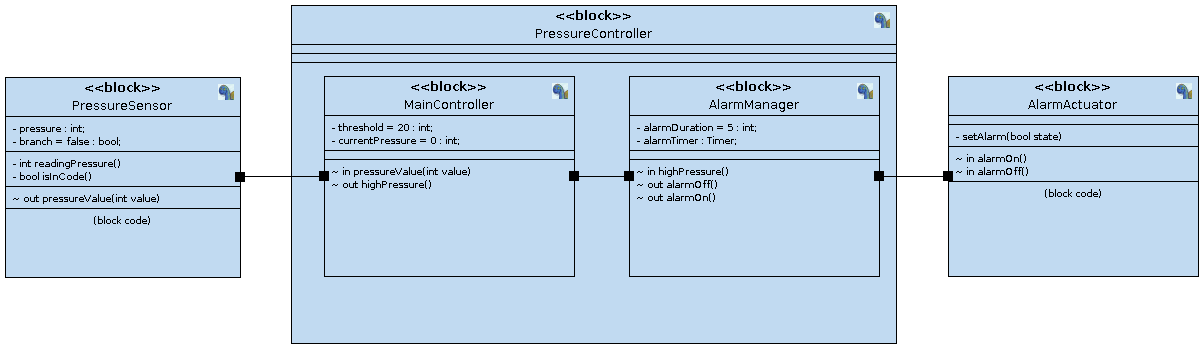
\includegraphics[width=1\textwidth]{images/PressureController.png}
\caption{Pressure Controller System: Avatar Design}
\label{fig:pressurecontroller}
\end{figure}

\subsubsection{PressureSensor}
The pressure sensor (see Figure \ref{fig:pressuresensor}) monitors the pressure with a period of 20 units of time. In the first branch, "IsInCode" method is \textbf{not} executed when the model is considered for functional simulation or formal verification. Indeed, in our case, the "branch" boolean is set to false by default, so the random command is executed (and not the readingPressure() method). The random value, between 18 and 21, is sent every period of time to the main controller.

\begin{figure}[h!]
\centering
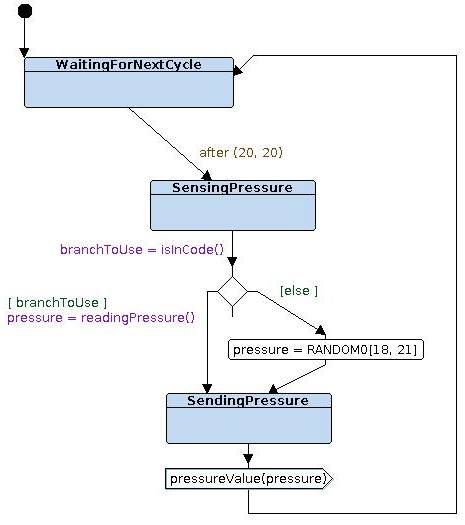
\includegraphics[width=0.6\textwidth]{images/pressuresensor.jpg}
\caption{Pressure Sensor}
\label{fig:pressuresensor}
\end{figure}

\subsubsection{MainController}
The main controller (see Figure \ref{fig:maincontroller}) receives the pressure value from the pressure sensor. If the value is greater equal than a threshold, set at 20, a high pressure signal is sent to the alarm manager.

\begin{figure}[h!]
\centering
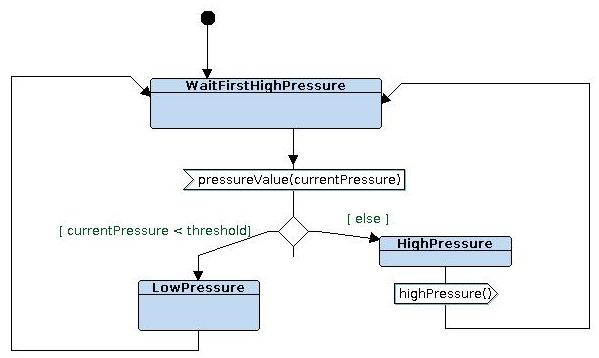
\includegraphics[width=0.7\textwidth]{images/maincontroller.jpg}
\caption{Main Controller}
\label{fig:maincontroller}
\end{figure}

\subsubsection{AlarmManager}
The alarm manager (see Figure \ref{fig:alarmmanager}) activates an alarm when the controller senses a high pressure. The alarm is deactivated after "alarmDuration", controlled by a timer, if no other high pressure signals are sensed in the meanwhile.

\begin{figure}[h!]
\centering
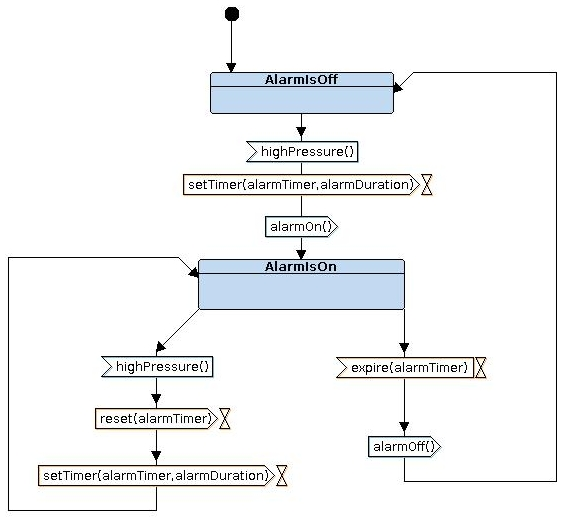
\includegraphics[width=0.7\textwidth]{images/alarmmanager.jpg}
\caption{AlarmManager}
\label{fig:alarmmanager}
\end{figure}

\subsubsection{AlarmActuator}
The alarm actuator may receive on and off signals activating and deactivating the alarm.


\subsection{Reachability and liveness}
To activate the reachability and liveness check for specific states, we need to go to the correspondant block state machine, right click on a state or a signal and select "Check for Reachability / Liveness". For instance, let's do that on the \textit{AlarmIsOn} state in the AlarmManager state machine. After this operation, the letters R and L in grey will appear next to the state (see Figure \ref{fig:rl_grey}) to confirm that the state is selected for the reachability and liveness check. After that, we may proceed with the verification.
\begin{figure}[h!]
\centering
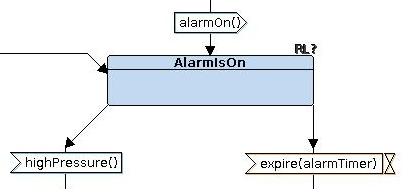
\includegraphics[width=0.5\textwidth]{images/rl_grey.jpg}
\caption{State selected for reachability and liveness check}
\label{fig:rl_grey}
\end{figure}
\\To open the model-checker window, we must first compile the model. To do that, let's click on the "syntax analysis" icon and then on "check syntax". Then, we click on the "safety verification (internal tool)" icon representing a screwdriver and a wrench crossed with the text "RC". The following window should open (see Figure \ref{fig:mcwindow}).
\begin{figure}[h!]
\centering
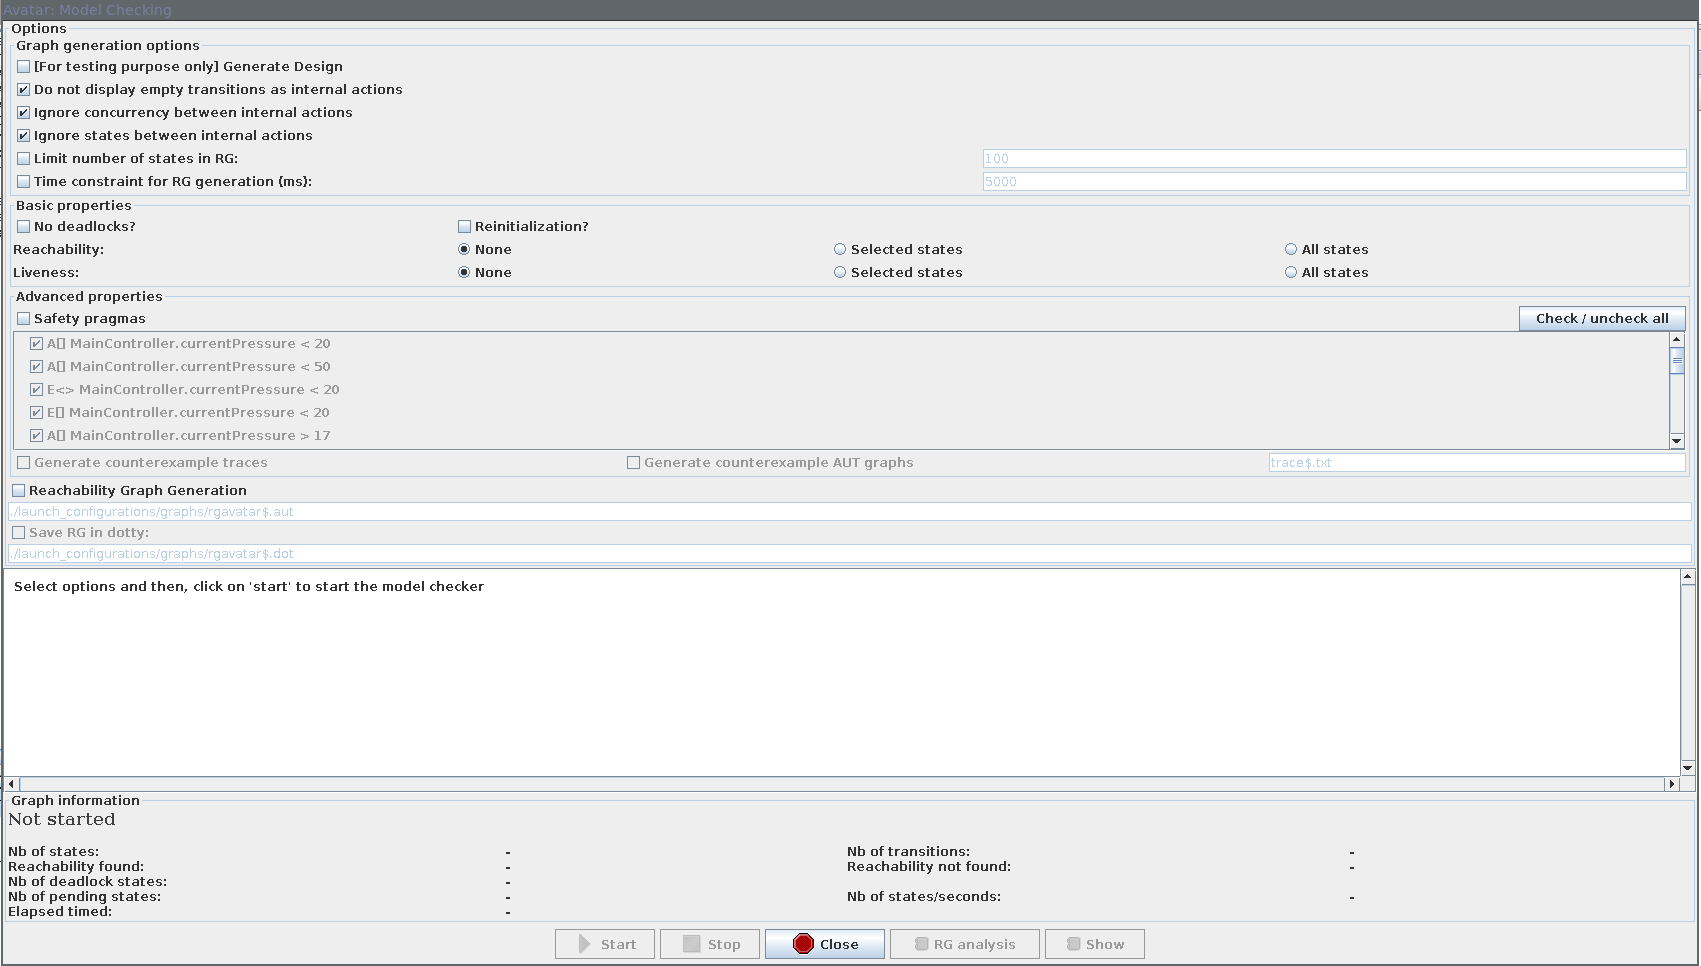
\includegraphics[width=\textwidth]{images/modelcheckerwindow.jpg}
\caption{Model-checker window}
\label{fig:mcwindow}
\end{figure}
\\To execute the reachability and liveness check on the selected state, let's select "Selected states" in both Reachability and Liveness lines. Then, we can press the start button. The text area will contain the verification report indicating if the properties are satisfied or not. Moreover, if we go back to the AlarmManager state machine, the RL text next to the state is now colored with green for \textit{satisfied} and in red for \textit{not satisfied} (see Figure \ref{fig:rl_exe}).
\begin{figure}[h!]
\centering
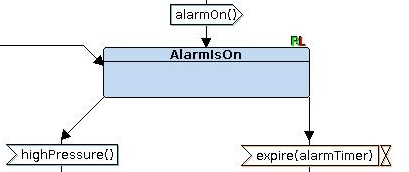
\includegraphics[width=0.5\textwidth]{images/rl_exe.jpg}
\caption{Reachability and Liveness result}
\label{fig:rl_exe}
\end{figure}
\\In this case, the reachability is satisfied as the pressure sensor may detect a temperature higher than the controller threshold. The liveness, instead, is not satisfied as a temperature higher than the threshold may be never detected.
\\\\
If we want to simply verify the reachability and liveness property automatically for all the states, we can select "All states" in the model-checking window.

\subsection{Safety properties}
We can find, write and modify safety properties in the block diagram tab inside the pink block. The pink block can be created by clicking on the "Safety property button" as shown in figure \ref{fig:safety}.
\begin{figure}[h!]
\centering
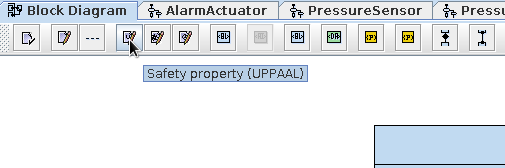
\includegraphics[width=0.6\textwidth]{images/safety.png}
\caption{Safety properties creation}
\label{fig:safety}
\end{figure}
\\If we do a double click on the pink box, we see the safety and liveness pragmas written as a CTL formula using UPPAAL syntax. If we press the question mark in the window, a short illustrated guide on how the queries work appears.
\\\\
To start the CTL query verification, let's compile again and let's open the model-checker window. As shown in figure \ref{fig:mcwindow}, we want to select the checkbox "Safety pragmas" and then we select the queries that we want to verify. In this case, let's execute all of them. Let's press the start button to begin the verification. The query results are shown both in the report field and inside the pink box in the block diagram tab (see Picture \ref{fig:sresult}).
\begin{figure}[h!]
\centering
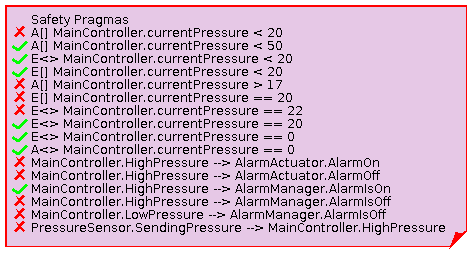
\includegraphics[width=0.7\textwidth]{images/safety_result.png}
\caption{Safety Result}
\label{fig:sresult}
\end{figure}

\newpage
\section{Verification Guide} \label{sec:vg}
In this section we will explain all the features and options that are present in the AVATAR model-checker. For a reference to the model-checking window, please refer to figure \ref{fig:mcwindow}.
\\\\The model-checker allows to generate a reachability graph and to prove properties. Starting from the top, the first section contains graph generations options. In particular:
\begin{itemize}
	\item \textbf{Do not display empty transitions as internal states}: in the reachability graph generation, states are not created for empty transitions (no action, no time, no choice). In practice, empty transition states are collapsed together. This option does not affect the verification. Option on by default.
	\item \textbf{Ignore concurrency between internal actions}: this option allows to ignore a full concurrency study. It is very useful to limit the state explosion of the model due to all the concurrencies among its states. It is so suggested to keep it selected to have a faster verification. This option, however, affects only in the \textit{leadsto} study, and the reachability graph generation. \textbf{Important}: basic concurrency it is evaluated also with this optimization selected. Basic concurrency means that concurrency is normally evaluated until states with multiple transitions, or if statement, or signals communication are encounted. In normal usage, you should not need to deselect this option (example in the next section \ref{sec:cb}). Option on by default.
	\item \textbf{Ignore states between internal actions}: This option allows to ignore intermediate states between actions that can be directly executed. this optimization helps decreasing the number of states in the reachability graph generation. If  \textit{Ignore concurrency between internal actions} is not selected, this option automatically deactivated. We suggest to keep this option selected for verification as it would not affect the result. Option on by default.
	 \item \textbf{Limit the number of states in RG}: it limits the reachability graph generation to a fixed number of states. It is particularly useful for big models. This option is automatically ignored when a verification study is selected.
	 \item \textbf{Time constraint for RG generation}: it allows to stop the reachability graph generation after a fixed number of milliseconds. It is particularly useful for big models. This option is automatically ignored when a verification study is selected.
\end{itemize}
The next section contains options for basic properties verification:
\begin{itemize}
	\item \textbf{No deadlocks}: it checks that the model is deadlock free
	\item \textbf{Reinitialization}: it checks that, for all the paths, the model will eventually restart to the initial state
	\item \textbf{Reachability}: it checks for states reachability
	\item \textbf{Liveness}: it checks for states liveness
\end{itemize}
The next section allows to execute safety and liveness pragmas written as a CTL formula. Each of them can be selected or not for the verification.
\\\\
Then, \textbf{Reachability Graph Generation} options is used to generate and save the reachability graph. Moreover, it can can be saved also in "dotty" format.

\subsection{CTL query syntax}
The query syntax for CTL formulas, for expressions \texttt{p} and \texttt{q}, is the following:
\begin{itemize}
	\item \textbf{A[] p}: property p is always true for each path (other common notation \textbf{AG p})
	\item \textbf{A<> p}: property p will eventually be true for each path (other common notation \textbf{AF p})
	\item \textbf{E[] p}: there exists at least one path in which property p is always true (other common notation \textbf{EG p})
	\item \textbf{E<> p}:  there exists a path in which property p will eventually be true (other common notation \textbf{EF p})
	\item \textbf{p --> q}: whenever p is true, then q will eventually be true at some subsequent moment (other common notation \textbf{G(p $\Rightarrow$ Fq)})
\end{itemize}
Expression \texttt{p} and \texttt{q} may be on states or variables. The format used to reference a variable or a state of a block is \textit{BlockName.AttributeName} or \textit{BlockName.StateName}. Conditions on variables can be combined using classic C code like boolean operators (||, \&\&, and, or). Variables can be negated or inverted (not(variable)). Examples:
\begin{itemize}
	\item \textit{E<> Passenger.isInCockpit ==true \&\& DoorAndLockButton.inside==1}: there exists a path in which there is at least one state in which Passenger.isInCockpit is true and DoorAndLockButton.inside is equal to 1
	\item \textit{A[] MainController.currentPressure < 25}: MainController.currentPressure is always less than 25
	\item \textit{DoorAndLockButton.IN\_EMERGENCY\_CALL --> DoorAndLockButton.CLOSED\_AND\_LOCKED || DoorAndLockButton.CLOSED\_AND\_UNLOCKED}: whenever DoorAndLockButton.IN\_EMERGENCY\_CALL state is encounted, then or DoorAndLockButton.CLOSED\_AND\_LOCKED or DoorAndLockButton.CLOSED\_AND\_UNLOCKED will be encounted at some subsequent moment.
\end{itemize}

\subsection{Concurrency behavior} \label{sec:cb}
In section \ref{sec:vg}, we discussed about the option \textit{Ignore concurrency between internal actions} and how it could effect the model-checker behavior. In this section, we will show with a guided example the differences between having this option on or off.
\\\\
In this simplified example (see Figure \ref{fig:cb}), we have two blocks: a sensor and a main block that receive the informations.
\begin{figure}[h!]
\centering
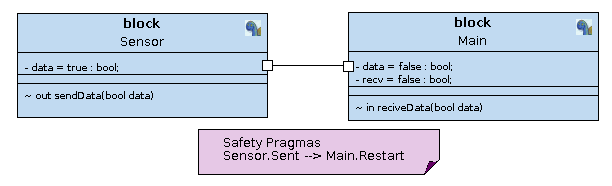
\includegraphics[width=0.8\textwidth]{images/conc_blocks.png}
\caption{Example on concurrency}
\label{fig:cb}
\end{figure}
Let's consider the two blocks connected through a synchronous channel. Also with asynchronous there would not be any difference in this analysis. The two states machine are shown in figure \ref{fig:csm}.
\begin{table}[h!]
	\begin{center}
	\begin{tabular}{ c c }
	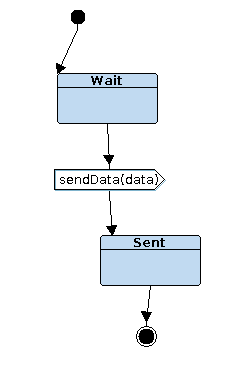
\includegraphics[scale=0.6]{images/conc_sensor.png}
	&
	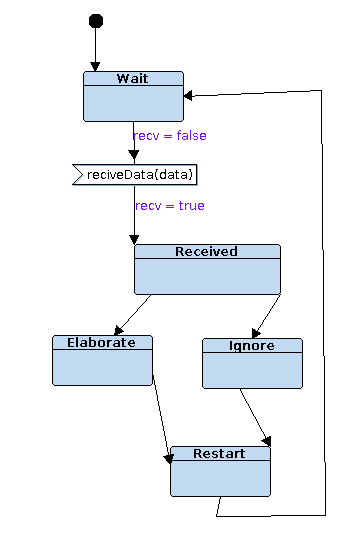
\includegraphics[scale=0.6]{images/conc_main.png}
	\\
	(a)
	&
	(b)
	\end{tabular}
	\end{center}
	\captionof{figure}{Sensor (a) and Main (b) state machines}
	\label{fig:csm}
\end{table}\\\\
First, we want to prove that after Sensor.Sent, Main will eventually reach the Receive state (\textit{Sensor.Sent --> Main.Receive}). After the data is sent by the sensor and received by the main block, the is a concurrency between executing first the Sent state or the Received state. In this case, both with the option \textit{Ignore concurrency between internal actions} selected or not, the pragma result will be always false. In fact, the Received state may be reached before Sent.\\
Different is the case for the following pragma: \textit{Sensor.Sent --> Main.Restart}. In this case, after the Received state, there are two possible choices: Elaborate and Ignore. If the option \textit{Ignore concurrency between internal actions} is selected, the single transitions have priority over the choices. This will lead to Sent being reached before Elaborate or Ignore. The pragma will be true. If the option is not selected instead, a full concurrency study is executed and the pragma will result correctly false. Note that a full concurrency study will considerably slow down the verification performance.
\\\\
The best way to avoid concurrency problems and to keep this option always selected is to ask concurrency aware queries. If we want to check if something happens after sending the data, the best choice would be to query \textit{Sensor.Wait --> Main.Restart}. This query does not depend by concurrency since it happens before a "synchronization" point.

\newpage
\section{AVATAR Model-Checker}
\label{sec:am}

\subsection{Introduction}
The model-checker is used to generate a reachability graph starting from an AVATAR model. It can be also used to check the reachability and liveness on a list of selected states. The model checker is contained inside the package \texttt{avatartranslator.modelchecker}.




\subsection{Reachability Graph}
The model-checker constructor takes an Avatar specification as input. The main method used for the graph generation is \texttt{startModelChecking()}. This method is responsible for preparing the data structure for the main algorithm to be executed. In particular, it runs the following operations:

\begin{itemize}
\item Remove else guards, timers, composite states, randoms from the state machine of blocks in the Avatar specification
\item Prepare the states
\item Prepare the transitions
\item Run \texttt{startModelChecking(nbThreads)}
\end{itemize}
The states are prepared inside the method \texttt{prepareStates()}. For each block inside the avatar specification, the method extracts all the states definitions (instances of \texttt{AvatarStateElement}) from the list of state machine elements \texttt{elements} saving them in the array \texttt{allStates}.

Transition between states of the state machines, instead, are prepared inside the method \texttt{prepareTransitions()}. This method is responsible for storing the type of transaction based on the type of the following state they address. The method is executed over all the blocks of the specification. The transitions are differentiated into the following categories:
\begin{itemize}
\item TYPE\_RECV\_SYNC
\item TYPE\_SEND\_SYNC
\item TYPE\_ACTION\_AND\_METHOD
\item TYPE\_ACTIONONLY
\item TYPE\_METHODONLY
\item TYPE\_EMPTY
\end{itemize}
Then the number of available processors is stored and passed to the next method \texttt{startModelChecking(nbThreads)}.




\subsection{Main algorithm preparation}
\label{sec:am_prep}
The reachability graph generation starts in the method \texttt{startModelChecking(nbThreads)}. In the first part, the graph data structures are initialized:
\begin{itemize}
\item \texttt{states}: map used to store the states of the reachability graph (\texttt{SpecificationState}), mapped by the hash of the state
\item \texttt{statesByID}: map used to store the states of the reachability graph (\texttt{SpecificationState}), mapped by the ID (incremented every time a state is created)
\item \texttt{pendingStates}: list of graph states that can be executed during the current iteration of the algorithm
\end{itemize}
The initial state of the reachability graph is created. A (\texttt{SpecificationState}  saves all the current configuration of the blocks and state machines. This is reached wrapping the Avatar blocks into specification blocks. SpecificationBlock adds an integer array saving:
\begin{itemize}
\item \textbf{State}: it points the current state of the state machine of the wrapped block in \texttt{allStates}
\item \textbf{Clock\_min}: minimum value of the current clock used as a lower bound to extract the executable transitions (time domain)
\item \textbf{Clock\_max}: maximum value of the current clock used as a higher bound to extract the executable transitions (time domain)
\item \textbf{Attributes}: values of block variables
\end{itemize}
The initial state is initialized storing the specification blocks for each Avatar Block. Specification blocks are initialized with the start state, clock at 0 and with initial variables value.\\

The method \texttt{handleNonEmptyUniqueTransition()} is used to increase the current state of specification block until not empty unique transitions are found. For instance, if from the initial state of the state machine there is only one empty (true guard, no time, no signal, no action) transition to another state, it can be directly executed since it doesn't have any dependency. Executing first these transitions helps to decrease the number of states created in the reachability graph.\\

Then a hash for the state is created. All the specification block states values (state, clock, values) are stored together in an array called \texttt{hash}. For this array, a hash number is calculated. The initial state is then inserted inside the maps \texttt{states}, \texttt{statesByID} and inside the \texttt{pendingStates} list.\\

Then the method \texttt{computeAllStates()} is called to run the main algorithm on multiple threads.

\subsection{The Main Algorithm}
The main loop of the algorithm is run in parallel by multiple threads in the method \texttt{run()}. The main loop executes the following actions:
\begin{itemize}
\item Pick-up a state from the pending state queue
\item Prepare the transitions from the selected state
\item Execute the valid available transitions
\item Gather the next possible states
\item Create a link in the reachability graph between current and new states
\item Insert the new states in the pending list
\end{itemize}
A state is picked up with the method \texttt{pickupState()}. The thread waits for an available state to be processed in the pendent queue.\\

The main method for the application of the algorithm is \texttt{computeAllStatesFrom(SpecificationState)}. 
First it prepares the transitions from the current state with the method \texttt{prepareTransitionsOfState(specificationState)}. For a specification state, it creates an array \texttt{transitions} containing all the possible transitions that could be executed from the current specification state, i.e. from the states pointed by the specification blocks for each state machine, wrapped in specification transitions. \\
The method \texttt{handleAvatarTransition} checks if a transition can be executed at the current state. First, it checks if the guard condition is satisfied. Then it wraps the transition under analysis inside a specification transition. A specification transition saves the following information:
\begin{itemize}
\item If the start state of the transition (state machine) has multiple transitions
\item The transition of the state machine which is represented
\item The  min and max clock values
\end{itemize}
The minimum and maximum clock of the transaction are calculated. A transition can happen during a time contained inside an interval\footnote{A trasition may occur after max clock value has elapsed in case the following action is not possible, e.g. waiting for a signal that is not yet available}. Inside these clock variables we want to store the difference from the current time interval for a transition to occur:
\begin{itemize}
\item The minimum clock value would be given by the situation when the past transition occurs as late as possible and the current under analysis happens as soon as possible (assuming that this transition starts after the past one)
\item The maximum clock value would be given by the situation when the past transition occurs as soon as possible and the current under analysis happens as late as possible (assuming that this transition starts after the past one)
\item When the assumption (the transition starts after the past one) is not valid, the reasoning is exactly the opposite
\end{itemize}
This interval is important as only transitions within the smallest interval can be executed (exhaustive explanation further on in the documentation).\\

Then, the main method selects the executable transitions of the specification state base on the following criteria:
\begin{itemize}
\item A synchronous transition (Send, Receive) is executable if both the sender and the receiver transitions, which belong to the same signal, are available in \texttt{transitions}.
\item Only the first available transitions can be executed. The minimum clock depends on the transition with the minimum clock min. The maximum clock, instead, by the first transition with the minimum max clock. For instance, let's imagine that we are at clock (0, 0) and we have three transitions (0, 3), (1, 2), (4, 5). In this case, the min clock will be 0 and max clock 2. The two possible transitions that can be executed are (0, 3) and (1, 2)
\item Each transition is limited by the general max clock
\end{itemize}
The \texttt{ignoreConcurrenceBetweenInternalActions} flag controls the possibility of executing as soon as possible empty transitions with no alternatives and no time constraints. For all the transitions that follow these rules, the method \texttt{computeAllInternalStatesFrom} is called.\\

First of all, a new state \texttt{newState} is created from a copy of the current one. Then it is updated with new values depending on the transition. The first operation is to update the clock time for each specification block. The time is kept relative to the past transition. So, after a transition is executed, the specification block where the transition occurred will have min and max time at zero. For instance, let's execute a transition A. After transition A, a transition B can happen with a delay between 20 and 30 units. No matter the value of the clock before transition A, the clock is set at 0 to wait for an interval of time between 20 and 30. For specification blocks not in the transitions, instead, the current clock has to be increased and then upper bounded to the max clock of the transition. For instance, let's take a transition A on SP1 with time (10, 20), a transition B on SP2 with time (20, 30), and a global clock at 0. After transition A is executed. The clock in SP2 is increased becoming (10, 20) so that the time is considered advancing during transition A.\\

The transition is executed in the method \texttt{executeTransition}. The next state pointed by the transition is retrieved, the state index of the specification block is updated, and the action or the synchronized signal is executed.\\

The hash of the newly created state is then used to check if an already existing state with the same configuration already exists. In this case, only a link would be added and the new state copy will be deleted.\\

For nonempty transitions, in general, the execution procedure is the same as the algorithm's preparation explained in subsection \ref{sec:am_prep} which is executed for all the pendent transitions. Continuing the main loop of the algorithm, the global reachability graph can be generated.


\section{Reachability of States}
The reachability condition of states is checked while creating the reachability graph. The array \texttt{reachabilities} contains the states elements to be checked. Every time a transition is executed, from state $s_t$ to state $s_{t+1}$, $s_{t+1}$ is checked for reachability. When all the states elements in \texttt{reachabilities} have been reached or the reachability graph is completed, the reachability study finishes.

\section{Safety and Liveness}
\subsection{Definitions}
In the model also safety and liveness conditions could be proved. In particular, imagining a structure in time of the model, as a tree, the following CTL and LTL formulas are supported:
\begin{itemize}
	\item \textbf{A[] p}: property p is always true for each path (other common notation \textbf{AG p})
	\item \textbf{A<> p}: property p will eventually be true for each path (other common notation \textbf{AF p})
	\item \textbf{E[] p}: there exists at least one path in which property p is always true (other common notation \textbf{EG p})
	\item \textbf{E<> p}:  there exists a path in which property p will eventually be true (other common notation \textbf{EF p})
	\item \textbf{p --> q}: whenever p is true, then q will be true at some subsequent moment (other common notation \textbf{G(p $\Rightarrow$ Fq}))
\end{itemize}
with \textit{p} and \textit{q} properties. \textbf{Properties are written as expressions on variables or states of the AVATAR model}.

\subsection{Handling of safety and liveness properties by the AVATAR model checker}
Safety and liveness properties are represented by the \texttt{SafetyProperty} class. The properties are built in the AvatarExpressionSolver class. It creates a syntax tree where each leaf is a AvatarExpressionAttribute or an immediate value and each node is an operator. An AvatarExpressionAttribute can represent a state or a variable of the model. It contains pointers so that, given a state of the model checker, it extracts the associated value in \textit{O(1)}. It can represent integers and boolean values encoded as integers. So, results of properties can be extracted just by visiting the AvatarExpressionSolver tree. AvatarExpressionSolver is also used for guards and actions. The methods \texttt{getSolverResult(SpecificationState)} and \texttt{getSolverResult(SpecificationState, AvatarStateMachineElement)} can be use to obtain the expressions result.\\

Safety properties are solved by finding loops or terminal conditions (deadlocks) in the model. For each property type we now explain how the modelchecker behaves.
\begin{itemize}
	\item \textbf{A[] p}: if during the reachability graph creation, $p$ is false is a new state new state has p false, then the property is false.
	\item \textbf{A<> p}: if the property is true for a state, stop the search on that path. If a false loop or a false deadlock is found, the property is false. If no false loops or false deadlocks are found, the property is true.
	\item \textbf{E[] p}:  if the property is false for a state, stop the search on that path. If a true loop or a true deadlock is found , the property is true. If no true loops or false deadlocks are found, the property is false.
	\item \textbf{E<> p}:  if during the reachability graph creation, $p$ is true in a new state,  then the property is true.
	\item \textbf{p --> q}: every time \texttt{p} is true save the SpecificationState in the safetyLeadStates array. Then, for each node in safetyLeadStates start a liveness check \texttt{A<>p} from that node. If the liveness is true for all the nodes in safetyLeadStates or safetyLeadStates is empty, the property is true, else it is false.
\end{itemize}

\subsection{Handling combinatory explosion}
The exploration space of states explodes easily in many models. That's why proving properties is hard. The basic idea of liveness is to find a counter example to prove it wrong. So, we want to detect a cycle (or a path that ends to a deadlock) for which the state we want to check is not live. If the states space explodes, an exploration in breadth will not be effective as the number of nodes increases too much before proving or disproving any property, the space will be too big to be explored.\\

Moreover, loops are found analyzing a path in depth. So, the check is executed in a depth first search-like manner, instead of a breadth first search implemented for other types of studies, like reachability. It will allow us to search through a path for a property to be true or false having a result within a manageable states  space most of the times. As soon as a property is (un)satisfied the search can continue through another path or stop. In the implementation, each thread follows a path to disprove the liveness. As soon as the property is unsatisfied, the check can stop. As soon as the property is satisfied, the search in that path can stop, and another one is fetched.\\

\end{document}
